%Pre - Post SIRS

\chapter{An investigation into the relationship between preoperative clinico-pathological characteristics and post-operative systemic inflammatory response in patients undergoing pancreaticoduodenectomy.}
\label{ch_pre_post_sirs}

\lhead{Chapter \ref{ch_pre_post_sirs}. \emph{Factors affecting post-operative systemic inflammation}} % This is for the header on each page - perhaps a shortened title
\clearpage

%----------------------------------------------------------------------------------------

\section{Introduction}
The perioperative systemic inflammatory response has a significant role in determining short-term and long-term outcomes following potentially curative surgery for a wide variety of cancers. 
Systemic inflammation both before and after major surgery has been reported to be associated with significant morbidity. 

Elevated preoperative systemic inflammation was associated with increased complications after colorectal surgery \parencite{moyes_preoperative_2009, kubo_elevated_2013}, oesophagectomy \parencite{vashist_glasgow_2010} as well as liver surgery for colorectal metastases \parencite{neal_preoperative_2011}. 
The modified Glasgow Prognostic Score in particular, which uses the combination of C-reactive protein and serum albumin, has been reported to be associated with increased incidence of complications \parencite{moyes_preoperative_2009, mohri_correlation_2014, vashist_glasgow_2010}.
Elevated preoperative CRP levels have also been reported to be associated with increased incidence of complications including infections and renal dysfunction as well as increased in-hospital mortality after cardiac surgery \parencite{lorenzo_increased_2012, mezzomo_preoperative_2011, kim_predictive_2009, biancari_preoperative_2003, boeken_increased_1998}.

Moreover, an elevated postoperative systemic inflammatory response in the first few days after surgery was associated with increased incidence of infective complications after a wide variety of thoraco-abdominal procedures \parencite{singh_systematic_2014, platt_c-reactive_2012, dutta_persistent_2011, welsch_persisting_2008} as well as other types of surgery \parencite{mcneer_early_2010, laporta_baez_c-reactive_2011}.
%Include some recent reviews pp singh, bjs as well as check Donny's email.
The magnitude of this postoperative inflammatory response has also been reported to be associated with the severity of the complications \parencite{mcsorley_postoperative_2015}. 

In patients undergoing pancreaticoduodenectomy, preoperative systemic inflammation may be affected by several factors. 
These include the presence of obstructive jaundice with or without cholangitis, preoperative biliary intervention including endoscopic retrograde cholangio-pancreatography for diagnosis or biliary drainage and in some patients acute or chronic pancreatitis either due to obstruction of the main pancreatic duct or due to other causes. 
The effect of this `priming' of the immune system on postoperative outcomes is poorly understood in this cohort of patients. 

Chronic inflammation is also a recognised feature of obesity which is increasingly common in patients undergoing major surgery for pancreatic and other gastro-intestinal cancers. 
The impact of obesity, especially visceral obesity, on complications after pancreaticoduodenectomy remains controversial with some authors reporting that obesity was associated with increased incidence of complications \parencite{house_preoperative_2008, ramsey_body_2011} while others reporting similar outcomes in obese and non-obese patients \parencite{khan_does_2010, tsai_impact_2010, balentine_obesity_2011}. 

More recently, levels of adipocytokines, inflammatory mediators produced exclusively in adipose tissue, have been reported to be associated with postoperative surgical site infections after colorectal \parencite{ortega-deballon_preoperative_2013, matsuda_preoperative_2009} and gastric cancer surgery \parencite{yamamoto_association_2013}.
Sarcopenia has also been reported to be associated with  elevated postoperative systemic inflammation after colorectal surgery \parencite{reisinger_sarcopenia_2015}.
This emphasises the importance of adipose tissue metabolism and body composition in the preoperative systemic inflammatory status of surgical patients. 

To our knowledge, the relationship between the preoperative systemic inflammatory response and the magnitude of the postoperative systemic inflammatory response after pancreaticoduodenectomy has not been examined before. 
While obstructive jaundice in itself has recently been reported to have no effect on postoperative complications, the impact of preoperative obstructive jaundice on postoperative systemic inflammation has not been previously reported. 
Moreover, the relationship between comorbidity, body composition and aerobic capacity as measured by cardiopulmonary exercise testing and postoperative systemic inflammation has not been studied. 

\subsection{Aim}
The aim of this study was to examine the relationship between patient factors including preoperative systemic inflammation, obstructive jaundice, cardiopulmonary exercise test parameters and body composition and the magnitude of the postoperative systemic inflammation during the first week after a pancreaticoduodenectomy. 

%Post-operative CRP levels have been reported to be associated with the magnitude of surgery as well as to predict infectious complications after neurosurgery \parencite{al-jabi_value_2010}. 

\clearpage
\section{Patients and methods}

\subsection{Patients}
Patients who underwent elective pancreaticoduodenectomy between January 2008 and December 2012 at the West of Scotland Pancreatic Unit at the Glasgow Royal Infirmary were included in this study. 
Patients who underwent only a trial dissection or palliative surgical bypass for unresectable disease during this period were excluded.

\subsection{Preoperative data}
Routine preoperative blood tests including full blood count, liver function tests and serum C-reactive protein were performed in all patients on the day before surgery. 
These blood tests were also repeated every day for at least the first postoperative week. 
These results were collected from the hospital laboratory database using an automated MS Access application as outlined in Appendix \ref{AppendixAccessDatabase}. 

The modified Glasgow Prognostic Score (mGPS) was calculated as shown in Table \ref{table:mGPS} on page \pageref{table:mGPS} in Chapter \ref{ch_intro}. 
%The neutrophil-lymphocyte ratio was calculated by dividing the preoperative neutrophil count by the preoperative lymphocyte count and a threshold of 5.0 was used to dichotomise this variable. 
Standard thresholds were used to categorise other biochemical parameters. 
Obstructive jaundice was defined as serum bilirubin $>$35 $\mu$mol/L while severe obstructive jaundice was defined as serum bilirubin $>$250 $\mu$mol/L. 

\subsection{BMI and body composition}
Body Mass Index (BMI) was categorised using the World Health Organisation thresholds as shown in Table \ref{table:bmi_who} on p \pageref{table:bmi_who} in Chapter \ref{ch_intro}. 
Only one patient had a BMI less than 18.5 kg/m$2$ and was excluded from analysis involving BMI.
Body composition was calculated in a subset of these patients using preoperative computed tomography of the abdomen. 
The methodology used in the calculation of the individual components of body composition including visceral fat, subcutaneous fat and skeletal muscle is described in detail in Section \ref{sec:bodycomp_calculation} on page \pageref{sec:bodycomp_calculation}. 
Continuous data were converted into categorical data using tertiles.

\subsection{Comorbidity and CPET}
The Scottish Index of Multiple Deprivation (SIMD) Quintile Scores were calculated from the post-code of the patient's primary residence and dichotomised into two groups with scores of 1-3 and 4-5 respectively.
Lower scores indicated greater deprivation.
The POSSUM Physiology Score was calculated based on 11 physiological parameters (cardiac disease including hypertension, ischaemic heart disease and heart failure, respiratory disease causing breathlessness on exertion and COPD, ECG changes, pulse rate, blood pressure, haemoglobin, white cell count, serum sodium, serum potassium, serum urea and Glasgow Coma Scale) as described in Table \ref{table:intro_possum} on page \pageref{table:intro_possum}.

In patients who underwent cardiopulmonary exercise testing, $\dot{V}_{O_2}$AT and $\dot{V}_{O_2}$Peak were compared against postoperative systemic inflammation. 
$\dot{V}_{O_2}$AT was dichotomised using a value of 10 ml/kg/min while $\dot{V}_{O_2}$Peak was dichotomised using a value of 16 ml/kg/min. 
Cardiopulmonary exercise testing methodology has been described in Section \ref{sec:cpx_method} on page \pageref{sec:cpx_method}.


\subsection{Statistics}

Continuous variables are reported as median (inter-quartile range).
Non-parametric tests were used to compare postoperative inflammatory markers (continuous data) with preoperative clinico-pathological characteristics (categorical data). 
Mann-Whitney U test was used when two categories were present and Kruskal-Wallis test was used when more than two categories were present.

Line-plots were created comparing the trend of inflammatory markers during the first postoperative week with preoperative systemic inflammation, obstructive jaundice and $\dot{V}_{O_2}$AT with error bars representing 95\% confidence intervals. 

SPSS software (Version 22.0; IBM, USA) was used to perform statistical analysis. 
Effects were considered significant at $\alpha \leq0.05$. 

\clearpage
\section{Results}

\subsection{Clinico-pathological characteristics}

Pancreaticoduodenectomy was performed in 188 patients (126 male, 67\%) during the study period.
Preoperative C-reactive protein was elevated in 70 (37.6\%) patients while just over half the patients had a low preoperative serum albumin (96, 51.1\%). 
The modified Glasgow Prognostic Score revealed normal preoperative systemic inflammatory status (mGPS = 0) in 116 (62.4\%) patients, mild systemic inflammation in 16 (8.6\%) and severe inflammation in 54 (29.0\%) patients. 
Obstructive jaundice was present in 44 (23.4\%) patients and severe obstructive jaundice was present in 31 (16.5\%) patients. 
BMI data was available in 167 patients. 
More than half of these patients were overweight or obese with a BMI $>$ 25 in 87 (52.1\%) patients.
All the variables necessary for calculation of the POSSUM Physiology Score, a composite score of comorbidity and preoperative biochemistry, were available in 180 patients and it was elevated in 87 (48.3\%) patients.

The relationship between preoperative clinico-pathological characteristics and postoperative C-reactive protein levels (Tables \ref{table:sirs_crp} and \ref{table:sirs_crp_pvalues}), postoperative serum albumin (Tables \ref{table:sirs_alb} and \ref{table:sirs_alb_pvalues}) and postoperative neutrophil count (Tables \ref{table:sirs_neut} and \ref{table:sirs_neut_pvalues}) are presented.

\subsection{Preoperative vs. postoperative systemic inflammation}
The relationship between preoperative CRP and postoperative systemic inflammation is also depicted graphically in Fig. \ref{fig:sirs_crp}. 
The median CRP levels on the day of surgery and the first postoperative day (POD) were significantly higher in patients who had an elevated preoperative CRP. 
However, this association was not present after the first postoperative day.
%Elevated preoperative CRP was associated with a persistently lower serum albumin level for the entire duration of the first postoperative week (p$<$0.001 to p$<$0.002).
%It was also associated with a higher neutrophil count (p$<$0.01) from the 3$^{rd}$ to 6$^{th}$ postoperative days with a less but still significant association on the 7$^{th}$ postoperative day. 

Preoperative hypoalbuminemia on the other hand was associated with lower median postoperative CRP levels starting with POD 3. 
The median difference in postoperative CRP between patients with or without preoperative hypoalbuminemia was 30 mg/l on POD 3 (p$<$0.045) and 53 mg/l on POD 6 (p=0.002) with lower CRP levels in patients with hypoalbuminemia.
This relationship is shown in Fig. \ref{fig:sirs_alb_crp}.
%Preoperative hypoalbuminemia persisted postoperatively throughout the first week (p$<$0.001, Fig. \ref{fig:sirs_alb_alb}).
%There was no relationship between preoperative serum albumin levels and postoperative neutrophil count (Fig. \ref{fig:sirs_alb_neut}).

The trend in postoperative CRP appeared to differ depending on whether preoperative CRP and albumin were independently deranged.
Fig. \ref{fig:sirs_crp_crp_alb} and Table \ref{table:sirs_crp_with_alb} on page \pageref{fig:sirs_crp_crp_alb} show the results of this analysis.
When both preoperative CRP and preoperative albumin were normal, the trend in postoperative CRP is shown by the solid line (Line 0 in Fig. \ref{fig:sirs_crp_crp_alb}). 
When preoperative CRP was elevated in the presence of a normal preoperative albumin, postoperative CRP levels were significantly elevated and remained elevated during the first postoperative week (Line 1 in Fig. \ref{fig:sirs_crp_crp_alb}). 
However, hypoalbuminemia was associated with lower postoperative CRP levels regardless of whether preoperative CRP was normal (Line 2 in Fig. \ref{fig:sirs_crp_crp_alb}) or elevated (Line 3 in Fig. \ref{fig:sirs_crp_crp_alb}). 

\subsection{Obstructive jaundice vs. postoperative inflammation}
Obstructive jaundice was associated with significant differences in the postoperative systemic inflammatory response. 
Postoperative serum albumin levels were lower in jaundiced patients with severely jaundiced patients having the lowest levels (p$<$0.001, Fig. \ref{fig:sirs_bil_alb}). 
There were no significant changes in the trends of albumin levels and it is likely that preoperative hypoalbuminemia persisted postoperatively in these patients. 

However, the trends in postoperative CRP were significantly different between the jaundiced and non-jaundiced patients. 
Obstructive jaundice was associated with a significantly lower peak CRP on POD 2 (p=0.001) and this persisted until POD 6 (p=0.005, Table \ref{table:sirs_crp}, \ref{table:sirs_crp_pvalues}).
Median postoperative CRP had an inverse relationship with severity of preoperative obstructive jaundice (Fig. \ref{fig:sirs_bil_crp}).
Obstructive jaundice was associated with a delayed rise in the neutrophil count on POD 6 (p$<$0.05) and POD 7 (p$<$0.05) although this relationship was less significant (Fig. \ref{fig:sirs_bil_neut}). 

\subsection{CPET, comorbidity vs. postoperative inflammation}
Cardiopulmonary exercise testing was performed in 130 patients. 
$\dot{V}_{O_2}$AT could not be estimated in one patient.
$\dot{V}_{O_2}$AT was less than 10 ml/kg/min in 52 (40\%) of patients indicating reduced aerobic capacity in these patients.
There was no significant relationship between $\dot{V}_{O_2}$AT, $\dot{V}_{O_2}$Peak and postoperative CRP or neutrophil count. 
Serum albumin levels were lower in patients with $\dot{V}_{O_2}$AT$<$10 mls/kg/min (Fig. \ref{fig:sirs_at}).

There was no significant, persistent relationship between postoperative CRP and neutrophil count and preoperative neutrophil-lymphocyte ratio, SIMD score, body mass index, preoperative haemoglobin levels or the POSSUM Physiology score. 
However, postoperative hypoalbuminemia was associated with all the preoperative characteristics studied with the exception of BMI and SIMD (Tables \ref{table:sirs_alb} and \ref{table:sirs_alb_pvalues}).

\subsection{Body composition vs. postoperative inflammation}
Body composition data was available for 90 patients.
Visceral adipose tissue area (cm$^2$) was divided into tertiles as low (n=30, median 57.1 cm$^2$, IQR 29.0-62.4), moderate (n=30, 128.9 cm$^2$, 119.0-150.8) and high (n=30, 241.2 cm$^2$, 221.9-313.1). 
Subcutaneous adipose tissue area was divided into tertiles as low (n=30, median 94.1 cm$^2$, IQR 63.2-102.5), moderate (n=30, median 152.5 cm$^2$, IQR 141.3-175.3) and high (n=30, median 253.9 cm$^2$, IQR 203.2-290.3).
Skeletal muscle area was also divided into tertiles as low (n=30, median 96.7 cm$^2$, IQR 91.9-102.5), moderate (n=30, median 121.7 cm$^2$, IQR 116.4-130.9) and high (n=30, median 153.0 cm$^2$, IQR 145.3-167.6).

The relationship between body composition and postoperative CRP, albumin and neutrophil count is shown in Tables \ref{table:sirs_bodycomp_crp}, \ref{table:sirs_bodycomp_alb} and \ref{table:sirs_bodycomp_neut} respectively.
Postoperative CRP and neutrophil count were not related to any of the components of body composition aside from a weak linear association between neutrophil count on POD 2 and visceral fat area (p=0.046).
However, lower preoperative skeletal muscle area was associated with lower postoperative serum albumin on days 1 to 5 (all p$<$0.05).

\begin{sidewaystable}[p]
	\caption{The relationship  between postoperative CRP and preoperative clinico-pathological characteristics in patients undergoing pancreaticoduodenectomy. }
	\label{table:sirs_crp}
	\footnotesize
	\centering
	\renewcommand{\arraystretch}{1.2} %Increases space between rows
	%\setlength{\tabcolsep}{9pt} %sets the space between columns

	\begin{tabular}{|llr | cccccccc|}
		\hline
		Preop.              &           &   n &                                   \multicolumn{8}{c|}{Postoperative C-Reactive Protein}                                   \\
		variable            &           & 188 & Day 0      &     Day 1     &     Day 2     &     Day 3     &     Day 4     &     Day 5     &    Day 6     &     Day 7     \\ \hline
		CRP                 & $\leq$10  & 116 & 18 (11-31) & 115 (86-145)  & 214 (166-262) & 181 (132-245) & 142 (85-216)  & 114 (60-193)  & 109 (56-175) & 103 (55-175)  \\
		                    & $>$10     &  70 & 39 (26-56) & 151 (99-186)  & 211 (158-282) & 195 (145-252) & 152 (89-231)  & 114 (61-197)  & 105 (55-162) & 109 (50-172)  \\
		Albumin             & $\geq$35  &  92 & 25 (13-39) & 126 (95-157)  & 220 (165-279) & 205 (151-276) & 170 (103-241) & 131 (83-227)  & 140 (71-204) & 124 (72-192)  \\
		                    & $<$35     &  96 & 26 (14-44) & 119 (87-166)  & 204 (161-253) & 175 (124-237) & 134 (83-209)  & 101 (47-155)  & 87 (44-159)  &  88 (41-151)  \\
		mGPS                & 0         & 116 & 18 (11-31) & 115 (86-145)  & 214 (166-262) & 181 (132-245) & 142 (85-216)  & 114 (60-193)  & 109 (56-175) & 103 (55-175)  \\
		                    & 1         &  16 & 34 (25-72) & 164 (130-185) & 279 (196-304) & 229 (179-309) & 194 (128-281) & 164 (112-283) & 133 (77-226) & 127 (72-226)  \\
		                    & 2         &  54 & 39 (27-53) & 145 (95-186)  & 200 (152-248) & 179 (124-241) & 140 (79-216)  & 102 (58-153)  & 96 (54-159)  & 109 (44-154)  \\
		NLR                 & $\leq$5   & 159 & 24 (13-38) & 121 (88-161)  & 218 (165-270) & 186 (136-258) & 148 (85-226)  & 115 (60-197)  & 113 (56-175) & 117 (57-176)  \\
		                    & $>$5      &  29 & 43 (19-66) & 141 (95-167)  & 189 (152-232) & 160 (124-236) & 141 (92-189)  & 113 (67-144)  & 89 (54-149)  &  89 (50-119)  \\
		Bilirubin           & $\leq$35  & 113 & 25 (13-41) & 131 (95-165)  & 231 (180-275) & 204 (154-273) & 171 (102-237) & 127 (81-218)  & 121 (72-192) & 113 (71-175)  \\
		                    & 36-250    &  44 & 24 (14-43) & 124 (100-167) & 212 (167-277) & 182 (139-239) & 136 (90-203)  & 110 (51-139)  & 113 (48-163) & 103 (44-174)  \\
		                    & $>$250    &  31 & 28 (17-37) &  99 (67-128)  & 165 (116-202) & 149 (82-214)  &  95 (60-166)  &  59 (37-153)  & 55 (26-154)  &  70 (24-158)  \\
		BMI                 & $<25$     &  80 & 21 (12-42) & 121 (88-163)  & 207 (156-252) & 174 (132-242) & 134 (86-217)  & 105 (58-193)  & 87 (51-175)  &  92 (50-164)  \\
		                    & 25-29.9   &  64 & 26 (17-39) & 127 (93-164)  & 220 (187-269) & 203 (137-250) & 149 (86-201)  & 115 (62-164)  & 109 (55-165) & 110 (54-170)  \\
		                    & 30-34.9   &  23 & 34 (12-42) & 114 (90-133)  & 220 (148-270) & 205 (152-287) & 190 (97-230)  & 141 (67-222)  & 142 (55-181) & 136 (70-198)  \\
		                    & $>$35     &   9 & 31 (27-44) & 167 (116-178) & 204 (173-311) & 235 (147-293) & 210 (91-290)  & 167 (76-232)  & 172 (88-207) & 162 (148-178) \\
		%bmi                & $\leq$25  &  80 & 21 (12-42) & 121 (88-163)  & 207 (156-252) & 174 (132-242) & 134 (86-217)  & 105 (58-193)  & 87 (51-175)  &  92 (50-164)  \\
		%                   & $>$25     &  96 & 27 (17-40) & 124 (93-162)  & 220 (170-270) & 205 (148-266) & 164 (90-217)  & 118 (66-192)  & 117 (57-172) & 122 (57-175)  \\
		SIMD                & 4-5       &  61 & 26 (13-45) & 128 (98-168)  & 226 (183-271) & 208 (150-274) & 171 (108-231) & 127 (88-200)  & 137 (72-205) & 136 (71-220)  \\
		                    & 1-3       & 126 & 25 (14-39) & 121 (88-161)  & 207 (148-264) & 180 (132-242) & 140 (84-215)  & 105 (57-190)  & 94 (50-163)  &  98 (50-158)  \\
		$\dot{V}_{O_2}$AT   & $\geq$10  &  77 & 23 (12-40) & 118 (85-165)  & 222 (166-264) & 186 (132-252) & 148 (85-231)  & 111 (58-193)  & 106 (54-177) & 107 (51-173)  \\
		                    & $<$10     &  52 & 28 (19-41) & 121 (96-150)  & 222 (158-275) & 204 (151-262) & 175 (123-221) & 119 (80-204)  & 116 (63-174) & 113 (66-189)  \\
		$\dot{V}_{O_2}$Peak & $\geq$16 &  65 & 21 (12-37) & 106 (78-150)  & 214 (140-264) & 181 (132-235) & 150 (85-213)  & 110 (59-190)  & 113 (57-181) & 115 (51-175)  \\
		                    & $<$16     &  65 & 28 (19-44) & 123 (100-161) & 234 (173-279) & 214 (149-278) & 174 (92-237)  & 119 (63-204)  & 111 (57-172) & 111 (60-180)  \\
		Hb                  & $\geq$12  & 127 & 24 (13-38) & 116 (85-161)  & 214 (165-263) & 184 (136-247) & 151 (88-214)  & 111 (59-192)  & 102 (54-172) & 104 (51-174)  \\
		                    & $<$12     &  61 & 28 (18-45) & 140 (104-165) & 216 (163-279) & 186 (124-258) & 137 (89-231)  & 119 (64-197)  & 119 (63-170) & 106 (60-170)  \\
		PPS                 & $\leq$14  &  93 & 24 (13-36) & 116 (84-161)  & 205 (144-264) & 180 (129-242) & 131 (83-210)  & 107 (55-168)  & 104 (54-174) & 104 (52-174)  \\
		                    & $>$14     &  87 & 26 (14-45) & 128 (99-156)  & 214 (175-262) & 198 (136-255) & 158 (95-226)  & 118 (71-193)  & 114 (58-167) & 109 (53-173)  \\ \hline
	\end{tabular}	
\end{sidewaystable}
































\begin{table}[p]
	\caption{The relationship  between postoperative C-reactive protein and preoperative clinicopathological characteristics in patients undergoing pancreaticoduodenectomy: p-values only. }
	\label{table:sirs_crp_pvalues}
	\footnotesize
	\centering
	\renewcommand{\arraystretch}{1.2} %Increases space between rows
	%\setlength{\tabcolsep}{9pt} %sets the space between columns

	\begin{tabular}{|l | c c c c c c c c|}
		\hline
		Preop.              &         \multicolumn{8}{c|}{Postoperative C-Reactive Protein}          \\
		Variable            & Day 0    & Day 1    & Day 2 & Day 3 & Day 4 & Day 5    & Day 6 & Day 7 \\ \hline
		CRP                 & $<$0.001 & $<$0.001 & 0.669 & 0.522 & 0.741 & 0.831    & 0.789 & 0.834 \\
		Albumin             & 0.445    & 0.916    & 0.148 & 0.045 & 0.018 & 0.001    & 0.002 & 0.006 \\
		mGPS                & $<$0.001 & 0.001    & 0.037 & 0.048 & 0.084 & 0.029    & 0.215 & 0.347 \\
		NLR                 & 0.001    & 0.310    & 0.143 & 0.217 & 0.490 & 0.427    & 0.227 & 0.111 \\
		Bilirubin           & 0.869    & 0.009    & 0.001 & 0.001 & 0.003 & $<$0.001 & 0.005 & 0.072 \\
		BMI                 & 0.181    & 0.312    & 0.744 & 0.376 & 0.424 & 0.504    & 0.556 & 0.214 \\
		%BMI    01          & 0.057    & 0.910    & 0.325 & 0.135 & 0.474 & 0.375    & 0.426 & 0.166 \\
		SIMD                & 0.962    & 0.399    & 0.277 & 0.243 & 0.163 & 0.422    & 0.849 & 0.713 \\
		$\dot{V}_{O_2}$AT   & 0.042    & 0.749    & 0.838 & 0.587 & 0.330 & 0.448    & 0.659 & 0.389 \\
		$\dot{V}_{O_2}$Peak & 0.022    & 0.050    & 0.122 & 0.154 & 0.218 & 0.537    & 0.992 & 0.527 \\
		Haemoglobin         & 0.025    & 0.078    & 0.735 & 0.973 & 0.905 & 0.838    & 0.682 & 0.987 \\
		PPS                 & 0.114    & 0.192    & 0.525 & 0.308 & 0.127 & 0.338    & 0.954 & 0.919 \\ \hline
		\multicolumn{9}{l}{\textit{p} - Mann-Whitney U test or Kruskal-Wallis test}
	\end{tabular}	
	\vspace{1cm}

	
	\caption{The relationship  between postoperative serum albumin and preoperative clinicopathological characteristics in patients undergoing pancreaticoduodenectomy: p-values only. }
	\label{table:sirs_alb_pvalues}
		\begin{tabular}{|l | c c c c c c c c|}
			\hline
			Preop.              &                   \multicolumn{8}{c|}{Postoperative Serum Albumin}                    \\
			Variable            & Day 0    & Day 1    & Day 2    & Day 3    & Day 4    & Day 5    & Day 6    & Day 7    \\ \hline
			CRP                 & $<$0.001 & $<$0.001 & $<$0.001 & $<$0.001 & $<$0.001 & $<$0.001 & 0.001    & 0.002    \\
			Albumin             & $<$0.001 & $<$0.001 & $<$0.001 & $<$0.001 & $<$0.001 & $<$0.001 & $<$0.001 & $<$0.001 \\
			mGPS                & $<$0.001 & $<$0.001 & $<$0.001 & $<$0.001 & $<$0.001 & $<$0.001 & $<$0.001 & 0.001    \\
			NLR                 & $<$0.001 & $<$0.001 & 0.002    & 0.004    & 0.014    & 0.008    & 0.150    & 0.137    \\
			Bilirubin           & $<$0.001 & $<$0.001 & $<$0.001 & $<$0.001 & $<$0.001 & $<$0.001 & $<$0.001 & $<$0.001 \\
			BMI                 & 0.126    & 0.413    & 0.446    & 0.374    & 0.671    & 0.821    & 0.595    & 0.700    \\
			%BMI    01          & 0.068    & 0.153    & 0.169    & 0.116    & 0.238    & 0.378    & 0.221    & 0.406    \\
			SIMD                & 0.297    & 0.407    & 0.336    & 0.848    & 0.984    & 0.940    & 0.850    & 0.915    \\
			$\dot{V}_{O_2}$AT   & 0.020    & 0.010    & 0.024    & 0.022    & 0.012    & 0.019    & 0.024    & 0.068    \\
			$\dot{V}_{O_2}$Peak & 0.012    & 0.015    & 0.023    & 0.016    & 0.020    & 0.032    & 0.019    & 0.188    \\
			Haemoglobin         & $<$0.001 & $<$0.001 & $<$0.001 & $<$0.001 & $<$0.001 & $<$0.001 & 0.001    & 0.001    \\
			PPS                 & 0.002    & 0.001    & $<$0.001 & $<$0.001 & $<$0.001 & 0.001    & 0.019    & 0.014    \\ \hline
			\multicolumn{9}{l}{\textit{p} - Mann-Whitney U test or Kruskal-Wallis test}
		\end{tabular}
\end{table}

\begin{sidewaystable}[p]
	\caption{The relationship  between postoperative Albumin and preoperative clinico-pathological characteristics in patients undergoing pancreaticoduodenectomy. }
	\label{table:sirs_albumin}
	\footnotesize
	\centering
	\renewcommand{\arraystretch}{1.2} %Increases space between rows
	%\setlength{\tabcolsep}{9pt} %sets the space between columns

	\begin{tabular}{|llr | c c c c c c c c|}
		\hline
		Preop.              &           & n   &                           \multicolumn{8}{c|}{Postoperative Serum Albumin}                            \\
		variable            &           & 188 & Day 0      & Day 1      & Day 2      & Day 3      & Day 4      & Day 5      & Day 6      & Day 7      \\ \hline
		CRP                 & $\leq$10  & 116 & 19 (16-23) & 20 (18-23) & 20 (18-23) & 19 (17-22) & 20 (16-22) & 20 (17-23) & 20 (17-23) & 20 (17-24) \\
		                    & $>$10     & 70  & 16 (13-19) & 17 (14-21) & 17 (15-20) & 16 (14-19) & 16 (14-19) & 17 (15-19) & 17 (15-20) & 18 (15-22) \\
		Albumin             & $\geq$35  & 92  & 20 (18-23) & 22 (19-24) & 22 (20-23) & 20 (19-23) & 20 (18-23) & 21 (18-23) & 21 (19-24) & 21 (19-25) \\
		                    & $<$35     & 96  & 16 (13-19) & 16 (14-20) & 17 (14-19) & 16 (13-19) & 16 (14-19) & 16 (14-19) & 17 (15-20) & 17 (14-20) \\
		mGPS                & 0         & 116 & 19 (16-23) & 20 (18-23) & 20 (18-23) & 19 (17-22) & 20 (16-22) & 20 (17-23) & 20 (17-23) & 20 (17-24) \\
		                    & 1         & 16  & 20 (18-22) & 22 (19-23) & 21 (19-22) & 20 (18-22) & 19 (17-21) & 18 (17-23) & 20 (18-23) & 21 (17-24) \\
		                    & 2         & 54  & 14 (13-17) & 16 (14-18) & 16 (14-18) & 15 (13-19) & 15 (14-19) & 16 (14-18) & 16 (14-20) & 17 (14-20) \\
		NLR                 & $\leq$5   & 159 & 19 (15-22) & 20 (16-23) & 20 (17-22) & 19 (16-22) & 19 (15-22) & 19 (16-22) & 19 (16-23) & 20 (16-23) \\
		                    & $>$5      & 29  & 15 (12-18) & 17 (15-19) & 17 (15-20) & 16 (14-19) & 17 (14-19) & 17 (15-19) & 18 (16-20) & 19 (15-22) \\
		Bilirubin           & $\leq$35  & 113 & 20 (17-23) & 21 (18-24) & 21 (19-23) & 20 (18-22) & 20 (18-22) & 20 (18-23) & 20 (18-23) & 21 (18-23) \\
		                    & 36-250    & 44  & 16 (14-20) & 18 (14-21) & 17 (16-20) & 16 (15-19) & 17 (14-20) & 17 (15-22) & 18 (15-23) & 19 (15-23) \\
		                    & $>$250    & 31  & 14 (12-16) & 15 (13-17) & 15 (12-17) & 14 (12-16) & 14 (13-16) & 15 (13-17) & 15 (14-17) & 15 (13-19) \\
		BMI                 & $<25$     & 80  & 17 (14-20) & 19 (15-22) & 18 (16-22) & 18 (15-20) & 18 (15-21) & 18 (15-22) & 19 (15-22) & 19 (15-23) \\
		                    & 25-29.9   & 64  & 19 (14-21) & 20 (16-23) & 20 (16-23) & 19 (15-22) & 19 (16-21) & 19 (17-22) & 20 (17-22) & 20 (17-23) \\
		                    & 30-34.9   & 23  & 19 (16-23) & 19 (16-22) & 20 (17-22) & 19 (16-21) & 19 (16-21) & 20 (17-22) & 19 (17-22) & 20 (19-23) \\
		                    & $>$35     & 9   & 20 (17-23) & 19 (18-26) & 20 (18-22) & 19 (18-20) & 19 (17-20) & 17 (16-21) & 18 (16-20) & 18 (17-20) \\
		%bmi                & $\leq$25  & 80  & 17 (14-20) & 19 (15-22) & 18 (16-22) & 18 (15-20) & 18 (15-21) & 18 (15-22) & 19 (15-22) & 19 (15-23) \\
		%                   & $>$25     & 96  & 19 (15-22) & 19 (16-23) & 20 (17-22) & 19 (16-21) & 19 (16-21) & 19 (17-22) & 19 (17-22) & 20 (17-23) \\
		SIMD                & 1-3       & 87  & 19 (15-22) & 19 (16-23) & 20 (16-22) & 19 (15-21) & 19 (15-21) & 18 (15-21) & 19 (15-22) & 20 (15-23) \\
		                    & 4-5       & 100 & 18 (14-21) & 19 (15-22) & 19 (16-22) & 19 (16-22) & 19 (16-21) & 18 (16-22) & 19 (16-22) & 19 (16-23) \\
		$\dot{V}_{O_2}$AT   & $\geq$10  & 77  & 19 (16-23) & 20 (18-23) & 20 (18-22) & 19 (16-22) & 19 (16-21) & 19 (17-22) & 20 (17-22) & 20 (16-23) \\
		                    & $<$10     & 52  & 17 (13-20) & 18 (15-22) & 17 (15-22) & 16 (14-20) & 17 (14-21) & 17 (14-20) & 17 (14-20) & 18 (15-21) \\
		$\dot{V}_{O_2}$Peak & $\geq$160 & 65  & 20 (16-23) & 21 (17-23) & 20 (18-23) & 19 (16-22) & 19 (16-22) & 19 (17-23) & 20 (16-23) & 20 (16-23) \\
		                    & $<$16     & 65  & 18 (14-20) & 19 (15-21) & 18 (15-22) & 17 (15-20) & 18 (14-20) & 18 (15-20) & 18 (15-20) & 19 (15-22) \\
		Haemoglobin         & $\geq$12  & 127 & 19 (16-22) & 20 (17-23) & 20 (18-23) & 19 (17-22) & 19 (16-22) & 20 (17-23) & 20 (17-23) & 20 (17-24) \\
		                    & $<$12     & 61  & 16 (13-19) & 17 (14-20) & 17 (14-20) & 16 (13-19) & 16 (14-19) & 17 (14-18) & 17 (15-20) & 17 (15-21) \\
		PPS                 & $\leq$14  & 93  & 19 (16-23) & 20 (17-23) & 20 (18-23) & 19 (17-22) & 20 (16-22) & 20 (17-23) & 20 (16-23) & 21 (17-25) \\
		                    & $>$14     & 87  & 17 (14-20) & 18 (15-21) & 18 (15-21) & 16 (13-20) & 17 (14-20) & 17 (14-20) & 18 (15-22) & 19 (15-22)\\ \hline
	\end{tabular}	
\end{sidewaystable}






































\begin{sidewaystable}[p]
	\caption{The relationship  between postoperative serum albumin and preoperative clinicopathological characteristics in patients undergoing pancreaticoduodenectomy: p-values only. }
	\label{table:sirs_alb_pvalues}
	%\footnotesize
	\centering
	\renewcommand{\arraystretch}{1.2} %Increases space between rows
	%\setlength{\tabcolsep}{9pt} %sets the space between columns
	\begin{tabular}{|l | c c c c c c c c|}
		\hline
		Preop.              &                   \multicolumn{8}{c|}{Postoperative Serum Albumin}                    \\
		Variable            & Day 0    & Day 1    & Day 2    & Day 3    & Day 4    & Day 5    & Day 6    & Day 7    \\ \hline
		CRP                 & $<$0.001 & $<$0.001 & $<$0.001 & $<$0.001 & $<$0.001 & $<$0.001 & 0.001    & 0.002    \\
		Albumin             & $<$0.001 & $<$0.001 & $<$0.001 & $<$0.001 & $<$0.001 & $<$0.001 & $<$0.001 & $<$0.001 \\
		mGPS                & $<$0.001 & $<$0.001 & $<$0.001 & $<$0.001 & $<$0.001 & $<$0.001 & $<$0.001 & 0.001    \\
		NLR                 & $<$0.001 & $<$0.001 & 0.002    & 0.004    & 0.014    & 0.008    & 0.150    & 0.137    \\
		Bilirubin           & $<$0.001 & $<$0.001 & $<$0.001 & $<$0.001 & $<$0.001 & $<$0.001 & $<$0.001 & $<$0.001 \\
		BMI                 & 0.126    & 0.413    & 0.446    & 0.374    & 0.671    & 0.821    & 0.595    & 0.700    \\
		%BMI    01          & 0.068    & 0.153    & 0.169    & 0.116    & 0.238    & 0.378    & 0.221    & 0.406    \\
		SIMD                & 0.306    & 0.110    & 0.255    & 0.389    & 0.456    & 0.729    & 0.827    & 0.949    \\
		$\dot{V}_{O_2}$AT   & 0.020    & 0.010    & 0.024    & 0.022    & 0.012    & 0.019    & 0.024    & 0.068    \\
		$\dot{V}_{O_2}$Peak & 0.012    & 0.015    & 0.023    & 0.016    & 0.020    & 0.032    & 0.019    & 0.188    \\
		Haemoglobin         & $<$0.001 & $<$0.001 & $<$0.001 & $<$0.001 & $<$0.001 & $<$0.001 & 0.001    & 0.001    \\
		PPS                 & 0.002    & 0.001    & $<$0.001 & $<$0.001 & $<$0.001 & 0.001    & 0.019    & 0.014    \\ \hline
		\multicolumn{9}{l}{\textit{p} - Mann-Whitney U test or Kruskal-Wallis test}
	\end{tabular}
\end{sidewaystable}

\begin{sidewaystable}[p]
	\caption{The relationship  between postoperative neutrophil count and preoperative clinico-pathological characteristics in patients undergoing pancreaticoduodenectomy. }
	\label{table:sirs_neut}
	\footnotesize
	\centering
	\renewcommand{\arraystretch}{1.2} %Increases space between rows
	\setlength{\tabcolsep}{5pt} %sets the space between columns
	
	\begin{tabular}{|l l | cc cc cc cc |}
		\hline
		Preop.              & n         &                                             \multicolumn{8}{c|}{Postoperative Neutrophil Count}                                              \\
		Variable            & 188       & Day 0           &      Day 1      & Day 2            &      Day 3      & Day 4          &     Day 5      & Day 6           &      Day 7      \\ \hline
		CRP                 & $\leq$10  & 10.3 (7.8-13.1) & 10.4 (8.5-12.6) & 11.0 (8.9-13.9)  & 8.1 (6.3-10.7)  & 6.7 (4.8-9.2)  & 6.6 (4.9-9.5)  & 8.0 (6.1-10.8)  & 9.7 (7.4-13.3)  \\
		                    & $>$10     & 11.0 (9.1-14.0) & 11.2 (9.4-14.9) & 12.6 (9.1-15.8)  & 10.5 (7.1-13.3) & 7.8 (6.0-11.4) & 8.3 (6.6-11.1) & 10.4 (7.6-13.4) & 11.6 (8.4-15.2) \\
		Albumin             & $\geq$35  & 10.7 (8.3-13.5) & 10.7 (8.5-13.8) & 11.4 (8.9-15.1)  & 8.4 (6.6-12.1)  & 7.0 (5.1-9.6)  & 7.0 (5.1-9.8)  & 8.8 (6.2-11.6)  & 10.4 (7.1-13.4) \\
		                    & $<$35     & 10.4 (8.4-13.2) & 10.7 (8.7-13.7) & 12.0 (9.0-14.6)  & 8.7 (6.4-12.3)  & 7.6 (5.3-10.8) & 7.9 (5.6-10.9) & 9.4 (6.9-13.1)  & 10.5 (7.9-14.3) \\
		mGPS                & 0         & 10.3 (7.8-13.1) & 10.4 (8.5-12.6) & 11.0 (8.9-13.9)  & 8.1 (6.3-10.7)  & 6.7 (4.8-9.2)  & 6.6 (4.9-9.5)  & 8.0 (6.1-10.8)  & 9.7 (7.4-13.3)  \\
		                    & 1         & 10.0 (8.4-13.6) & 12.5 (7.8-15.2) & 13.2 (9.3-15.9)  & 10.6 (7.5-13.3) & 7.6 (5.2-10.5) & 7.7 (6.1-9.1)  & 9.6 (7.2-11.7)  & 10.6 (8.4-14.3) \\
		                    & 2         & 11.1 (9.1-14.2) & 11.2 (9.9-14.9) & 12.6 (9.1-15.7)  & 10.4 (7.1-13.3) & 8.1 (6.0-12.3) & 8.3 (6.8-11.2) & 10.8 (7.9-13.6) & 11.6 (8.4-15.7) \\
		NLR                 & $\leq$5   & 10.6 (8.3-13.5) & 10.9 (8.7-13.8) & 11.5 (8.9-14.6)  & 8.5 (6.4-12.0)  & 7.3 (5.2-10.0) & 7.4 (5.1-10.0) & 9.1 (6.2-12.4)  & 10.4 (7.7-13.7) \\
		                    & $>$5      & 10.5 (8.3-13.3) & 10.2 (7.9-13.2) & 12.6 (10.4-16.3) & 9.8 (7.1-12.3)  & 6.9 (5.2-11.4) & 7.1 (6.1-10.3) & 9.0 (7.2-12.9)  & 10.8 (8.3-13.6) \\
		Bilirubin           & $\leq$35  & 10.6 (8.3-13.7) & 10.7 (8.5-13.8) & 11.5 (8.9-14.8)  & 8.5 (6.7-12.0)  & 7.3 (5.2-9.6)  & 7.2 (5.1-9.5)  & 8.5 (6.4-11.3)  & 10.1 (7.7-13.4) \\
		                    & 36-250    & 10.4 (8.6-12.9) & 11.4 (8.6-14.5) & 11.2 (8.8-14.7)  & 7.9 (6.3-13.0)  & 6.5 (5.1-10.7) & 7.3 (5.6-9.7)  & 9.5 (6.3-13.1)  & 10.4 (7.2-13.8) \\
		                    & $>$250    & 10.8 (9.3-13.2) & 10.7 (9.5-13.2) & 12.1 (9.1-14.9)  & 9.6 (6.6-11.8)  & 7.8 (5.2-10.6) & 9.8 (5.6-13.9) & 11.3 (8.6-13.9) & 12.2 (8.9-18.5) \\
		BMI                 & $<25$     & 10.3 (8.4-12.8) & 10.6 (8.3-13.2) & 10.9 (8.4-14.1)  & 8.2 (6.4-11.8)  & 7.3 (5.0-10.1) & 7.4 (5.0-10.0) & 9.3 (6.9-12.3)  & 10.0 (7.3-13.7) \\
		                    & 25-29.9   & 11.1 (8.1-13.6) & 11.1 (8.5-14.9) & 12.4 (10.4-15.6) & 10.2 (7.1-12.5) & 7.6 (5.2-10.6) & 7.8 (6.1-10.0) & 9.0 (7.1-12.2)  & 10.5 (8.2-13.4) \\
		                    & 30-34.9   & 10.1 (7.6-13.0) & 10.3 (8.7-14.0) & 10.9 (8.7-15.7)  & 8.2 (6.2-12.1)  & 6.7 (5.5-9.0)  & 6.2 (5.0-7.9)  & 7.2 (5.7-11.0)  & 9.9 (6.3-13.8)  \\
		                    & $>$35     & 10.4 (9.7-14.0) & 10.7 (9.4-12.2) & 10.8 (10.0-12.1) & 10.3 (4.6-10.6) & 6.2 (4.4-9.7)  & 6.0 (5.1-11.4) & 8.0 (6.8-12.8)  & 12.8 (9.4-16.4) \\
		%bmi                & $\leq$25  & 10.3 (8.4-12.8) & 10.6 (8.3-13.2) & 10.9 (8.4-14.1)  & 8.2 (6.4-11.8)  & 7.3 (5.0-10.1) & 7.4 (5.0-10.0) & 9.3 (6.9-12.3)  & 10.0 (7.3-13.7) \\
		%                   & $>$25     & 10.7 (8.3-13.6) & 10.9 (8.7-14.6) & 12.0 (10.1-15.5) & 9.5 (6.7-12.3)  & 7.0 (5.3-10.5) & 7.4 (5.5-10.0) & 8.8 (6.7-12.0)  & 10.5 (8.1-13.4) \\
		SIMD                & 4-5       & 10.4 (8.3-12.9) & 11.3 (9.1-13.9) & 12 (9.4-15.7)    &  9 (6.9-13.4)   & 8 (6-11)       &  7.6 (5.5-11)  & 9 (7.1-13)      &  11.2 (8-13.7)  \\
		                    & 1-3       & 10.7 (8.4-13.9) & 10.5 (8.5-13.5) & 11.5 (8.8-14.5)  & 8.4 (6.4-11.6)  & 6.7 (5-9.6)    &  7.1 (5.1-10)  & 9 (6.2-12.2)    & 10.4 (7.7-13.7) \\
		$\dot{V}_{O_2}$AT   & $\geq$10  & 11.0 (8.8-13.7) & 11.2 (8.6-14.8) & 11.9 (9.4-14.8)  & 9.0 (6.7-12.3)  & 7.9 (5.7-9.9)  & 8.0 (5.7-10.3) & 9.4 (7.0-12.2)  & 11.2 (7.9-13.5) \\
		                    & $<$10     & 9.9 (7.6-12.7)  & 10.7 (8.0-13.7) & 12.1 (8.8-15.0)  & 9.1 (6.8-12.5)  & 7.2 (5.5-10.6) & 7.1 (5.3-10.0) & 8.9 (6.2-12.9)  & 10.4 (8.2-13.6) \\
		$\dot{V}_{O_2}$Peak & $\geq$160 & 10.9 (8.7-13.2) & 10.3 (8.5-13.8) & 11.9 (9.4-14.8)  & 8.9 (6.3-12.3)  & 7.8 (5.7-9.5)  & 7.9 (5.6-10.0) & 9.3 (6.9-12.3)  & 11.0 (7.7-14.1) \\
		                    & $<$16     & 10.0 (8.4-13.6) & 11.8 (8.5-14.7) & 12.1 (8.9-15.1)  & 9.4 (7.1-12.5)  & 7.8 (5.5-10.8) & 7.4 (5.3-10.3) & 9.3 (6.2-12.0)  & 10.4 (8.2-13.4) \\
		Hb                  & $\geq$12  & 10.5 (8.3-13.5) & 10.7 (8.4-13.8) & 11.3 (8.9-14.5)  & 8.4 (6.7-11.3)  & 7.2 (5.2-9.6)  & 7.3 (5.5-10.0) & 8.5 (6.4-12.0)  & 10.4 (7.7-13.7) \\
		                    & $<$12     & 10.8 (8.9-13.2) & 10.6 (9.5-13.9) & 12.4 (9.4-15.1)  & 9.6 (6.3-13.3)  & 7.0 (5.1-11.9) & 7.6 (5.2-10.8) & 9.8 (7.0-13.0)  & 10.9 (8.2-13.6) \\
		PPS                 & $\leq$14  & 10.5 (8.5-12.7) & 10.7 (8.7-13.0) & 10.9 (8.7-13.9)  & 8.1 (6.3-11.3)  & 6.8 (4.8-9.4)  & 7.2 (5.1-9.5)  & 8.4 (5.9-11.4)  & 10.1 (7.2-13.7) \\
		                    & $>$14     & 10.3 (7.5-13.7) & 10.5 (8.2-14.0) & 12.0 (9.4-15.7)  & 8.7 (6.6-12.8)  & 7.3 (5.3-10.8) & 7.6 (5.5-10.4) & 9.6 (7.1-13.1)  & 10.4 (8.2-13.6) \\ \hline
	\end{tabular}	
\end{sidewaystable}


























\begin{table}[p]
	\caption{The relationship  between postoperative neutrophil count and preoperative clinicopathological characteristics in patients undergoing pancreaticoduodenectomy: p-values only. }
	\label{table:sirs_neut_pvalues}
	%\footnotesize
	\centering
	\renewcommand{\arraystretch}{1.2} %Increases space between rows
	%\setlength{\tabcolsep}{9pt} %sets the space between columns
	\begin{tabular}{|l | c c c c c c c c|}
			\hline
			Preop.              &       \multicolumn{8}{c|}{Postoperative Neutrophil  Count}       \\
			Variable            & Day 0 & Day 1 & Day 2 & Day 3 & Day 4 & Day 5    & Day 6 & Day 7 \\ \hline
			CRP                 & 0.167 & 0.082 & 0.079 & 0.003 & 0.008 & $<$0.001 & 0.001 & 0.019 \\
			Albumin             & 0.911 & 0.901 & 0.586 & 0.572 & 0.280 & 0.097    & 0.070 & 0.302 \\
			mGPS                & 0.304 & 0.217 & 0.213 & 0.011 & 0.018 & 0.001    & 0.002 & 0.043 \\
			NLR                 & 0.832 & 0.259 & 0.253 & 0.366 & 0.699 & 0.697    & 0.729 & 0.661 \\
			Bilirubin           & 0.904 & 0.903 & 0.801 & 0.819 & 0.669 & 0.053    & 0.012 & 0.034 \\
			BMI                 & 0.614 & 0.762 & 0.134 & 0.469 & 0.904 & 0.382    & 0.602 & 0.826 \\
			%BMI    01          & 0.342 & 0.403 & 0.051 & 0.292 & 0.612 & 0.714    & 0.789 & 0.787 \\
			SIMD                & 0.305 & 0.555 & 0.596 & 0.507 & 0.541 & 0.328    & 0.877 & 0.711 \\
			$\dot{V}_{O_2}$AT   & 0.104 & 0.571 & 0.981 & 0.942 & 0.940 & 0.388    & 0.400 & 0.676 \\
			$\dot{V}_{O_2}$Peak & 0.441 & 0.481 & 0.689 & 0.335 & 0.529 & 0.720    & 0.664 & 0.711 \\
			Haemoglobin         & 0.682 & 0.590 & 0.230 & 0.225 & 0.462 & 0.639    & 0.122 & 0.969 \\
			PPS                 & 0.730 & 0.699 & 0.149 & 0.109 & 0.255 & 0.201    & 0.033 & 0.588 \\ \hline
			\multicolumn{9}{l}{\textit{p} - Mann-Whitney U test or Kruskal-Wallis test}
		\end{tabular}
\end{table}

\clearpage
%========================CRP vs Post-op SIRS============================================

\begin{figure}[p]
	\caption{Relationship between preoperative CRP levels and postoperative inflammatory markers in the first week after pancreaticoduodenectomy.}
	\label{fig:sirs_crp}
	\centering
	\begin{subfigure}{0.48\textwidth}
		\centering
		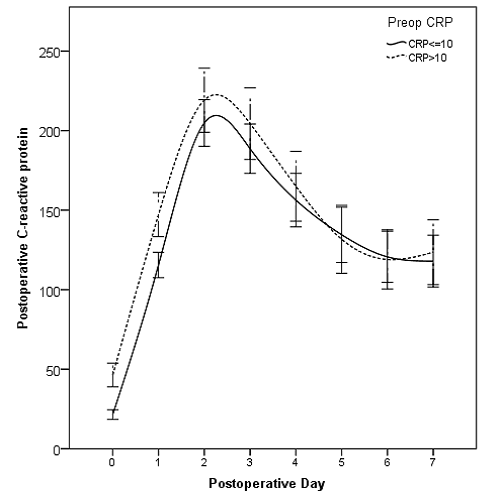
\includegraphics[width=\textwidth]{Figures/sirs_crp_crp}
		\caption{Preop. CRP vs. postop. CRP}
		\label{fig:sirs_crp_crp}
	\end{subfigure}
	\hfill
	\begin{subfigure}{0.48\textwidth}
		\centering
		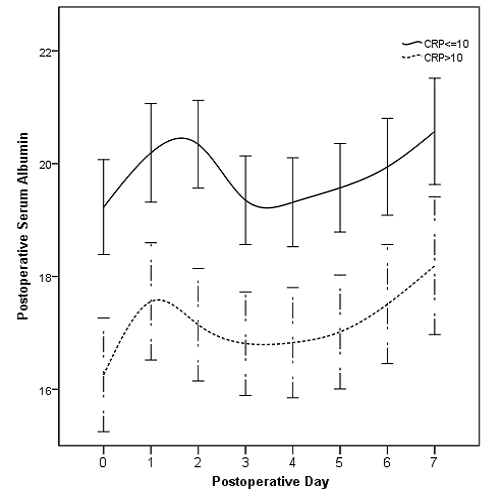
\includegraphics[width=\textwidth]{Figures/sirs_crp_alb}
		\caption{Preop. CRP vs. postop. Albumin}
		\label{fig:sirs_crp_alb}
	\end{subfigure}
	
	\vspace{1cm}
	
	\begin{subfigure}{0.48\textwidth}
		\centering
		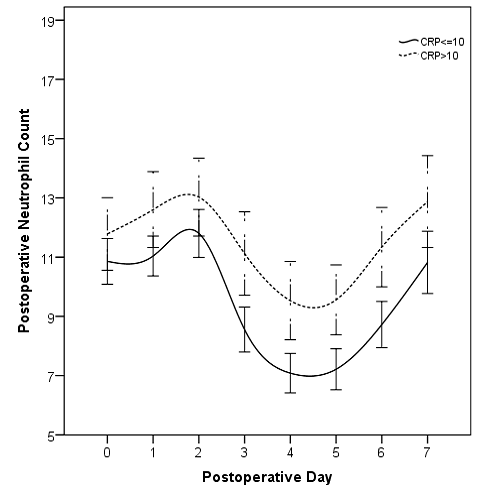
\includegraphics[width=\textwidth]{Figures/sirs_crp_neut}
		\caption{Preop. CRP vs. postop. Neutrophil count}
		\label{fig:sirs_crp_neut}
	\end{subfigure}	
\end{figure}
%==============================================================================

%========================Albumin vs Post-op SIRS============================================

\begin{figure}[p]
	\caption{Relationship between preoperative Albumin levels and postoperative inflammatory markers in the first week after pancreaticoduodenectomy.}
	\label{fig:sirs_alb}
	\centering
	\begin{subfigure}{0.48\textwidth}
		\centering
		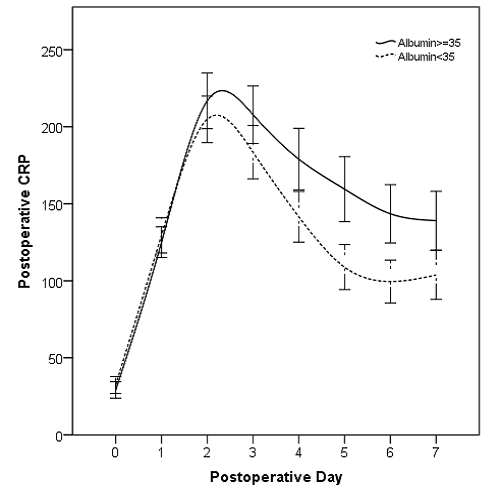
\includegraphics[width=\textwidth]{Figures/sirs_alb_crp}
		\caption{Preop. Albumin vs. postop. CRP}
		\label{fig:sirs_alb_crp}
	\end{subfigure}
	\hfill
	\begin{subfigure}{0.48\textwidth}
		\centering
		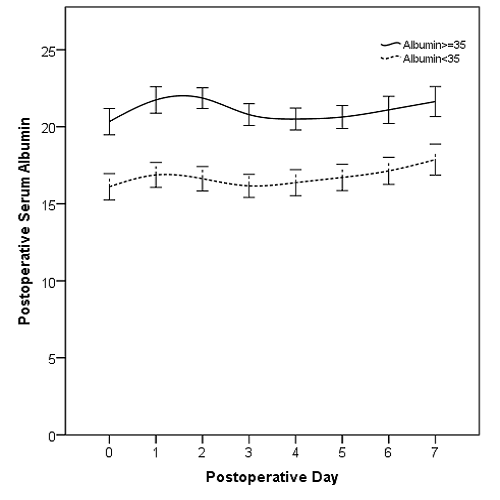
\includegraphics[width=\textwidth]{Figures/sirs_alb_alb}
		\caption{Preop. Albumin vs. postop. Albumin}
		\label{fig:sirs_alb_alb}
	\end{subfigure}
	
	\vspace{1cm}
	
	\begin{subfigure}{0.48\textwidth}
		\centering
		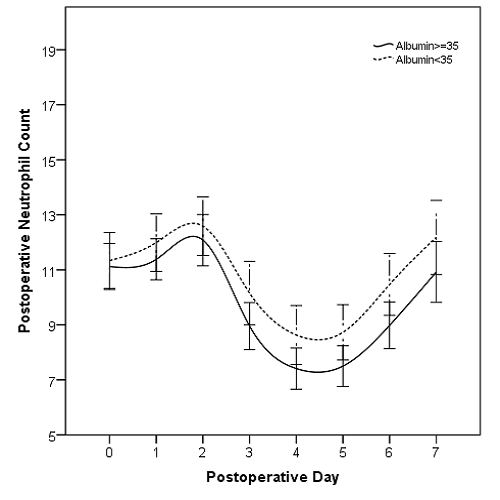
\includegraphics[width=\textwidth]{Figures/sirs_alb_neut}
		\caption{Preop. Albumin vs. postop. Neutrophil count}
		\label{fig:sirs_alb_neut}
	\end{subfigure}	
\end{figure}
%==============================================================================

%==============================================================================
\clearpage
\begin{figure}[t]
	\centering
	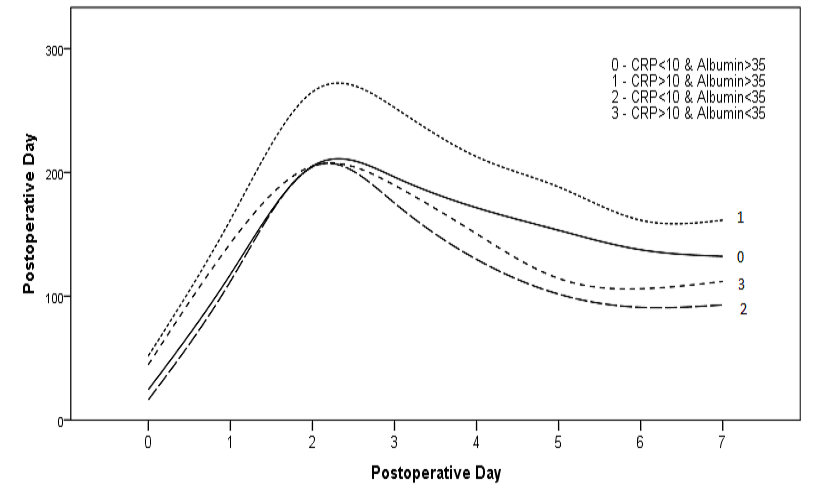
\includegraphics[width=\textwidth]{Figures/sirs_crp_crp_alb}
	\caption{Relationship between preoperative CRP and postoperative CRP in the presence or absence of preoperative hypoalbuminemia.}
	\label{fig:sirs_crp_crp_alb}
\end{figure}

\begin{table}[p]
	\caption{The relationship  between preoperative CRP and postoperative CRP in the presence or absence of preoperative hypoalbuminemia in patients undergoing pancreaticoduodenectomy. }
	\label{table:sirs_crp_with_alb}
	%\footnotesize
	\centering
	\renewcommand{\arraystretch}{1.4} %Increases space between rows
%	\setlength{\tabcolsep}{6pt} %sets the space between columns
	
	\begin{tabular}{|l c c c c c|}
		\hline
		      & \multicolumn{2}{c}{Preop Albumin $\geq$ 35 g/l} & \multicolumn{2}{c}{Preop Albumin $<$ 35 g/l} &  \\
		      & CRP $\leq$ 10 mg/l & CRP $>$ 10 mg/l            & CRP $\leq$ 10 mg/l & CRP $>$ 10 mg/l         & p        \\
		n     & 74                 & 16                         & 42                 & 54                      &  \\ \hline
		Day 0 & 21 (12-35)         & 34 (25-72)                 & 14 (10-19)         & 39 (27-53)              & $<$0.001 \\
		Day 1 & 122 (90-147)       & 164 (130-185)              & 110 (84-141)       & 145 (95-186)            & 0.002    \\
		Day 2 & 215 (155-268)      & 279 (196-304)              & 213 (168-257)      & 200 (152-248)           & 0.083    \\
		Day 3 & 198 (136-259)      & 229 (179-309)              & 174 (124-235)      & 179 (124-241)           & 0.056    \\
		Day 4 & 157 (97-238)       & 194 (128-281)              & 132 (83-184)       & 140 (79-216)            & 0.046    \\
		Day 5 & 129 (78-222)       & 164 (112-283)              & 95 (45-155)        & 102 (58-153)            & 0.003    \\
		Day 6 & 136 (66-195)       & 133 (77-226)               & 80 (38-167)        & 96 (54-159)             & 0.025    \\
		Day 7 & 123 (70-180)       & 127 (72-226)               & 76 (27-140)        & 109 (44-154)            & 0.037    \\ \hline
		\multicolumn{6}{l}{p - Kruskal-Wallis test}
	\end{tabular}	
\end{table}
\clearpage
%==============================================================================

%========================Bilirubin vs Post-op SIRS============================================

\begin{figure}[p]
	\caption{Relationship between obstructive jaundice and postoperative inflammatory markers in the first week after pancreaticoduodenectomy.}
	\label{fig:sirs_bilirubin}
	\centering
	\begin{subfigure}{0.48\textwidth}
		\centering
		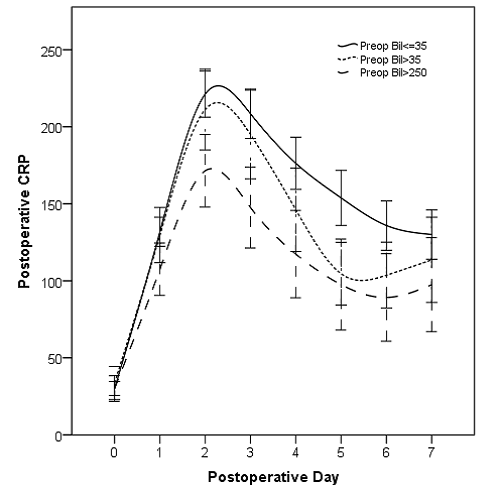
\includegraphics[width=\textwidth]{Figures/sirs_bil_crp}
		\caption{Preop. Bilirubin vs. postop. CRP}
		\label{fig:sirs_bil_crp}
	\end{subfigure}
	\hfill
	\begin{subfigure}{0.48\textwidth}
		\centering
		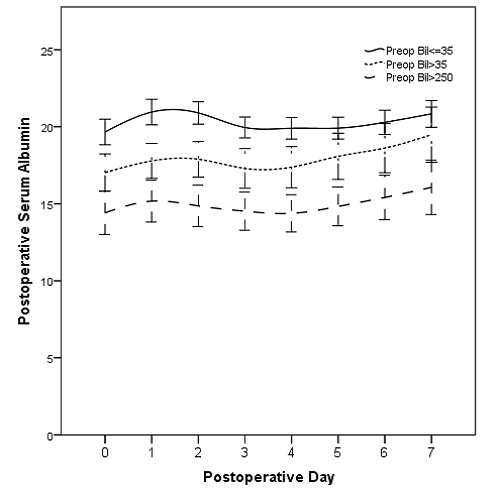
\includegraphics[width=\textwidth]{Figures/sirs_bil_alb}
		\caption{Preop. Bilirubin vs. postop. Albumin}
		\label{fig:sirs_bil_alb}
	\end{subfigure}
	
	\vspace{1cm}
		
	\begin{subfigure}{0.48\textwidth}
		\centering
		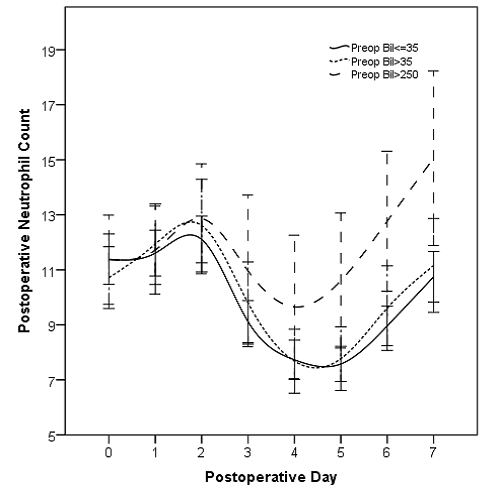
\includegraphics[width=\textwidth]{Figures/sirs_bil_neut}
		\caption{Preop. Bilirubin vs. postop. Neutrophil count}
		\label{fig:sirs_bil_neut}
	\end{subfigure}	
\end{figure}
%==============================================================================


%========================AT vs Post-op SIRS============================================

\begin{figure}[p]
	\caption{Relationship between $\dot{V}_{O_2}$AT and postoperative inflammatory markers in the first week after pancreaticoduodenectomy.}
	\label{fig:sirs_at}
	\centering
	\begin{subfigure}{0.48\textwidth}
		\centering
		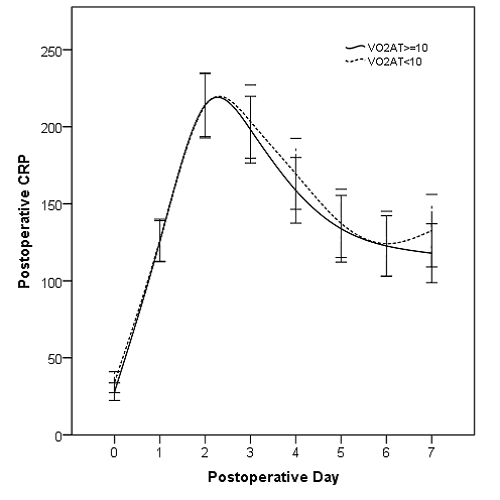
\includegraphics[width=\textwidth]{Figures/sirs_at_crp}
		\caption{Preop. $\dot{V}_{O_2}$AT vs. postop. CRP}
		\label{fig:sirs_at_crp}
	\end{subfigure}
	\hfill
	\begin{subfigure}{0.48\textwidth}
		\centering
		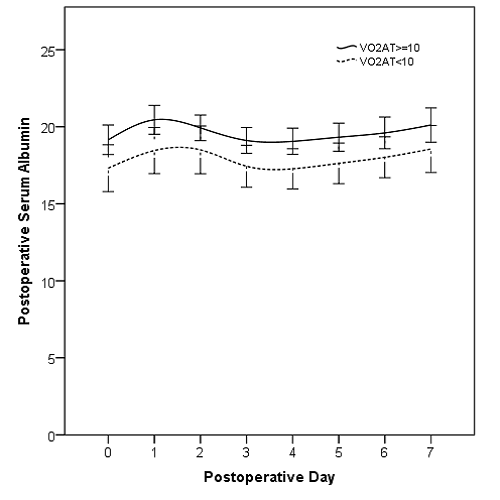
\includegraphics[width=\textwidth]{Figures/sirs_at_alb}
		\caption{Preop. $\dot{V}_{O_2}$AT vs. postop. Albumin}
		\label{fig:sirs_at_alb}
	\end{subfigure}
	
	\vspace{1cm}
		

	\begin{subfigure}{0.48\textwidth}
		\centering
		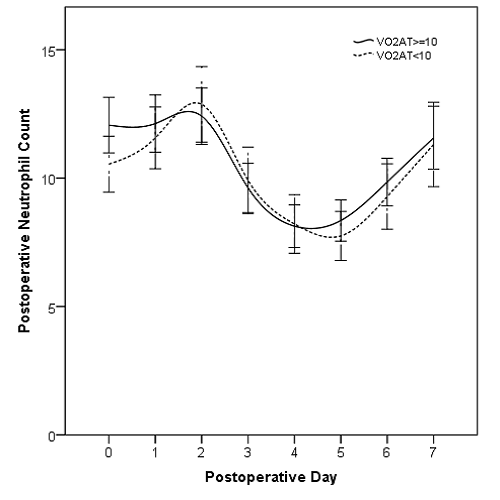
\includegraphics[width=\textwidth]{Figures/sirs_at_neut}
		\caption{Preop. $\dot{V}_{O_2}$AT vs. postop. Neutrophil count}
		\label{fig:sirs_at_neut}
	\end{subfigure}	
\end{figure}
%==============================================================================

\begin{table}[p]
	\caption{The relationship  between postoperative CRP and body composition in patients undergoing pancreaticoduodenectomy. }
	\label{table:sirs_bodycomp_crp}
	%\footnotesize
	\centering
	\renewcommand{\arraystretch}{1.2} %Increases space between rows
	\setlength{\tabcolsep}{9pt} %sets the space between columns
	
	\begin{tabular}{|l c c c c |}
		  \multicolumn{5}{c}{\textit{a.} Visceral fat vs. postoperative CRP}   \\ \hline
		      & Low           & Moderate      & High          & p              \\
		Day 0 & 22 (13-37)    & 26 (19-38)    & 30 (24-43)    & 0.161          \\
		Day 1 & 122 (89-179)  & 143 (108-165) & 121 (80-161)  & 0.374          \\
		Day 2 & 189 (155-261) & 244 (181-269) & 200 (152-245) & 0.326          \\
		Day 3 & 165 (104-214) & 202 (132-287) & 192 (136-248) & 0.161          \\
		Day 4 & 113 (69-216)  & 166 (85-239)  & 157 (129-210) & 0.409          \\
		Day 5 & 87 (45-176)   & 142 (59-200)  & 115 (95-168)  & 0.229          \\
		Day 6 & 75 (40-137)   & 148 (60-170)  & 146 (73-172)  & 0.167          \\
		Day 7 & 86 (31-141)   & 130 (64-174)  & 123 (66-175)  & 0.172          \\ \hline
		                         \multicolumn{5}{c}{}                          \\
		\multicolumn{5}{c}{\textit{b.} Subcutaneous fat vs. postoperative CRP} \\ \hline
		      & Low           & Moderate      & High          & p              \\
		Day 0 & 31 (19-44)    & 25 (15-33)    & 25 (18-42)    & 0.368          \\
		Day 1 & 132 (106-167) & 125 (68-168)  & 120 (99-153)  & 0.431          \\
		Day 2 & 216 (155-247) & 209 (181-278) & 226 (157-268) & 0.767          \\
		Day 3 & 156 (132-206) & 189 (110-273) & 217 (149-266) & 0.306          \\
		Day 4 & 132 (88-214)  & 159 (84-232)  & 157 (108-216) & 0.694          \\
		Day 5 & 105 (56-158)  & 115 (54-199)  & 121 (80-197)  & 0.690          \\
		Day 6 & 91 (40-147)   & 154 (56-170)  & 145 (76-174)  & 0.126          \\
		Day 7 & 95 (29-132)   & 117 (57-175)  & 136 (86-189)  & 0.089          \\ \hline
		                         \multicolumn{5}{c}{}                          \\
		\multicolumn{5}{c}{\textit{c.} Skeletal muscle vs. postoperative CRP}  \\ \hline
		      & High          & Moderate      & Low           & p              \\
		Day 0 & 27 (18-37)    & 24 (18-43)    & 25 (17-44)    & 0.951          \\
		Day 1 & 108 (78-167)  & 131 (109-188) & 140 (82-156)  & 0.090          \\
		Day 2 & 210 (155-278) & 223 (163-282) & 206 (162-245) & 0.382          \\
		Day 3 & 203 (149-273) & 174 (136-255) & 166 (104-241) & 0.356          \\
		Day 4 & 163 (117-218) & 145 (96-232)  & 132 (79-180)  & 0.304          \\
		Day 5 & 138 (80-197)  & 115 (82-213)  & 88 (40-163)   & 0.135          \\
		Day 6 & 156 (84-179)  & 121 (57-192)  & 94 (42-147)   & 0.080          \\
		Day 7 & 130 (77-178)  & 105 (64-151)  & 100 (33-165)  & 0.237          \\ \hline
		                         \multicolumn{5}{c}{}
	\end{tabular}
	\caption*{Patients were divided into three equal groups based on each component of body composition and the median CRP during the first postoperative after pancreaticoduodenectomy was compared between these groups using the Kruskal-Wallis test. 
	No relationship was identified between body composition and postoperative CRP levels. 
	Values are median (inter-quartile range) for postoperative CRP. }
\end{table}




\begin{table}[p]
	\caption{The relationship  between postoperative serum albumin and body composition in patients undergoing pancreaticoduodenectomy. }
	\label{table:sirs_bodycomp_alb}
	%\footnotesize
	\centering
	\renewcommand{\arraystretch}{1.2} %Increases space between rows
	\setlength{\tabcolsep}{9pt} %sets the space between columns
	
	\begin{tabular}{|l c c c c |}
		        \multicolumn{5}{c}{\textit{a.} Visceral fat vs. postoperative serum albumin}         \\ \hline
		      & Low        & Moderate   & High       & p                                             \\
		Day 0 & 18 (13-20) & 16 (13-20) & 19 (14-21) & 0.434                                         \\
		Day 1 & 18 (14-22) & 18 (14-20) & 20 (16-23) & 0.206                                         \\
		Day 2 & 18 (13-20) & 17 (15-20) & 20 (17-22) & 0.063                                         \\
		Day 3 & 17 (13-21) & 16 (14-19) & 20 (16-22) & 0.032                                         \\
		Day 4 & 16 (14-21) & 17 (14-20) & 20 (16-22) & 0.123                                         \\
		Day 5 & 17 (15-23) & 17 (14-20) & 20 (16-23) & 0.182                                         \\
		Day 6 & 16 (14-23) & 18 (15-22) & 20 (17-24) & 0.185                                         \\
		Day 7 & 18 (14-22) & 18 (15-23) & 21 (18-25) & 0.152                                         \\ \hline
		                                    \multicolumn{5}{c}{}                                     \\
		      \multicolumn{5}{c}{\textit{b.} Subcutaneous fat vs. postoperative serum albumin}       \\ \hline
		      & Low        & Moderate   & High       & p                                             \\
		Day 0 & 18 (13-20) & 19 (15-21) & 16 (13-19) & 0.091                                         \\
		Day 1 & 20 (15-22) & 20 (16-22) & 16 (14-19) & 0.024                                         \\
		Day 2 & 20 (15-22) & 20 (15-22) & 17 (14-20) & 0.099                                         \\
		Day 3 & 20 (15-22) & 19 (15-20) & 15 (12-19) & 0.040                                         \\
		Day 4 & 19 (14-22) & 19 (15-21) & 16 (13-19) & 0.090                                         \\
		Day 5 & 19 (14-23) & 19 (15-23) & 17 (14-18) & 0.244                                         \\
		Day 6 & 20 (16-24) & 18 (15-23) & 17 (15-20) & 0.322                                         \\
		Day 7 & 21 (17-25) & 20 (15-23) & 18 (15-20) & 0.333                                         \\ \hline
		                                    \multicolumn{5}{c}{}                                     \\
		      \multicolumn{5}{c}{\textit{c.} Skeletal muscle vs. postoperative serum albumin}        \\ \hline
		      & High       & Moderate   & Low        & p                                             \\
		Day 0 & 19 (15-21) & 18 (14-20) & 16 (12-19) & 0.070                                         \\
		Day 1 & 21 (16-23) & 18 (14-21) & 16 (14-20) & 0.042                                         \\
		Day 2 & 20 (17-23) & 18 (14-22) & 16 (14-20) & 0.006                                         \\
		Day 3 & 20 (15-22) & 18 (14-21) & 16 (13-19) & 0.046                                         \\
		Day 4 & 20 (16-22) & 18 (14-21) & 16 (13-19) & 0.046                                         \\
		Day 5 & 20 (16-23) & 18 (16-24) & 16 (13-19) & 0.013                                         \\
		Day 6 & 20 (16-22) & 18 (15-24) & 17 (14-22) & 0.143                                         \\
		Day 7 & 21 (17-23) & 20 (16-25) & 18 (13-22) & 0.073                                         \\ \hline
		                                    \multicolumn{5}{c}{}                                     \\
		\multicolumn{5}{l}{Values are median (inter-quartile range) for postoperative serum albumin}
	\end{tabular}	
\end{table}

		  
\begin{table}[p]
	\caption{The relationship  between postoperative neutrophil count and body composition in patients undergoing pancreaticoduodenectomy. }
	\label{table:sirs_bodycomp_neut}
	%\footnotesize
	\centering
	\renewcommand{\arraystretch}{1.2} %Increases space between rows
	\setlength{\tabcolsep}{9pt} %sets the space between columns
	
	\begin{tabular}{|l c c c c |}
		        \multicolumn{5}{c}{\textit{a.} Visceral fat vs. postoperative neutrophil count}         \\ \hline
		      & Low              & Moderate          & High              & p                            \\
		Day 0 & 9.55(7.1 -11.1)  & 10.7(8.7 -12.4)   & 9.3(7.3 -11.5)    & 0.224                        \\
		Day 1 & 10.2(8.2 -12.1)  & 10.35(9.7 -12.4)  & 11.1(7.9 -13.8)   & 0.792                        \\
		Day 2 & 10.15(7.9 -13.6) & 11.95(10.1 -14.8) & 12.7(9.4 -18.5)   & 0.046                        \\
		Day 3 & 7.85(6 -9.9)     & 9.6(7.5 -12.1)    & 10.35(7.6 -12.1)  & 0.075                        \\
		Day 4 & 6(4.5 -9)        & 8.2(5.4 -10.8)    & 8.35(6.2 -10.8)   & 0.149                        \\
		Day 5 & 7(4.7 -8.95)     & 8.05(5.5 -10)     & 7.1(5.5 -10)      & 0.528                        \\
		Day 6 & 8.2(5.9 -10.9)   & 8.8(6.9 -12.2)    & 8.65(6 -10.8)     & 0.784                        \\
		Day 7 & 8.9(7.4 -14.1)   & 10.5(8.1 -12.1)   & 10.2(8 -13.3)     & 0.904                        \\ \hline
		                                     \multicolumn{5}{c}{}                                       \\
		      \multicolumn{5}{c}{\textit{b.} Subcutaneous fat vs. postoperative neutrophil count}       \\ \hline
		      & Low              & Moderate          & High              & p                            \\
		Day 0 & 9.45(6.8 -11.2)  & 9.9(8.5 -11.8)    & 10.05(7.5 -13.5)  & 0.438                        \\
		Day 1 & 10.4(7.4 -12.3)  & 10.2(8.7 -12.1)   & 11.7(7.7 -13.8)   & 0.793                        \\
		Day 2 & 11.65(8.4 -14.2) & 11.35(8.8 -13.6)  & 13.2(9.4 -17.1)   & 0.206                        \\
		Day 3 & 8.35(6.9 -11.8)  & 8.5(7 -10.7)      & 10.2(7.1 -13.4)   & 0.381                        \\
		Day 4 & 7(4.5 -9)        & 7.65(5.1 -9.4)    & 7.95(5.6 -12)     & 0.247                        \\
		Day 5 & 6.95(4.9 -9.65)  & 7.3(5.1 -8.3)     & 7.75(5.5 -10.7)   & 0.247                        \\
		Day 6 & 8.35(6.1 -11)    & 7.45(5.95 -10.1)  & 9.6(6.7 -13)      & 0.168                        \\
		Day 7 & 10.45(7.7 -12.5) & 9.3(7.2 -13.35)   & 10.6(8.25 -13.65) & 0.475                        \\ \hline
		                                     \multicolumn{5}{c}{}                                       \\
		      \multicolumn{5}{c}{\textit{c.} Skeletal muscle vs. postoperative neutrophil count}        \\ \hline
		      & High             & Moderate          & Low               & p                            \\
		Day 0 & 9.5(8.4 -12)     & 9.55(6.9 -12)     & 10.2(8.5 -11.8)   & 0.707                        \\
		Day 1 & 10.55(8.2 -14.5) & 10.2(8 -12)       & 10.7(9.7 -13.4)   & 0.807                        \\
		Day 2 & 12.05(9.4 -16)   & 10.15(8.4 -13.6)  & 12.8(10.4 -15.1)  & 0.116                        \\
		Day 3 & 9.85(7.1 -11.8)  & 8.1(6.3 -12)      & 8.7(7.4 -11.8)    & 0.531                        \\
		Day 4 & 8.4(5.6 -10.6)   & 7.05(5.2 -10.2)   & 6.7(5.1 -10.4)    & 0.742                        \\
		Day 5 & 7.9(5.5 -10.2)   & 7.3(5.1 -9.5)     & 7.1(5.3 -9.8)     & 0.796                        \\
		Day 6 & 8.9(5.9 -12.8)   & 8.35(6.45 -11.7)  & 8.35(6.3 -10.9)   & 0.972                        \\
		Day 7 & 11.15(7.6 -14)   & 8.9(7.5 -12.45)   & 9.75(7.9 -13.45)  & 0.589                        \\ \hline
		                                     \multicolumn{5}{c}{}                                       \\
		\multicolumn{5}{l}{Values are median (inter-quartile range) for postoperative neutrophil count}
	\end{tabular}	
\end{table}








\clearpage
\section{Discussion}

The results of the present study demonstrate that preoperative systemic inflammation is associated with the magnitude of the postoperative systemic inflammatory response  in patients undergoing pancreaticoduodenectomy. 
The results also appear to show that preoperative obstructive jaundice is associated with a dampened systemic inflammatory response as measured by CRP levels. 
%However, neither aerobic capacity or the POSSUM Physiology Score were related to postoperative systemic inflammation. 
Taken together, these results appear to suggest that the preoperative inflammatory status of the patient plays an important role in modulating postoperative systemic inflammation which may not simply be due to the effect of surgery and its sequelae.

The role of postoperative CRP in predicting complications after surgery has been well established. 
A recent meta-analysis of six studies involving 1832 patients reported that CRP level less than 135 mg/l on the fourth postoperative day had a high negative predictive value of 89\% for infectious complications \parencite{warschkow_safe_2012}. 
Postoperative CRP has been shown to predict complications after pancreaticoduodenectomy by us (chapter \ref{ch_crp_comp}) as well as other authors \parencite{welsch_persisting_2008, hiyoshi_usefulness_2013, kosaka_multivariate_2014}.
The role of preoperative systemic inflammation as measured by the modified Glasgow Prognostic Score or the neutrophil-lymphocyte ratio has also been reported to be adversely affect long-term survival in patients undergoing potentially curative surgery in over a hundred studies involving a variety of gastrointestinal and non-gastrointestinal cancers. 

However, preoperative systemic inflammation as measured by elevated C-reactive protein or an abnormal modified Glasgow Prognostic Score is increasingly recognised as an independent risk factor for postoperative infectious complications \parencite{mohri_correlation_2014, kubo_elevated_2013, moyes_preoperative_2009}.

We hypothesized that preoperative systemic inflammation may adversely affect postoperative immuno-modulation resulting in an abnormal response in patients whose immune systems have been `primed' before the surgical insult. 
This may affect the healing processes as well as the patient's ability to clear endotoxins and may predispose the patient to infective and other complications.
The results of the present study appear to support this hypothesis. 

In this study, raised preoperative CRP in the absence of hypoalbuminemia was associated with elevated postoperative systemic inflammation.
However, preoperative hypoalbuminemia was associated with significantly lower levels of postoperative CRP.
These apparently opposite effects of preoperative CRP and albumin on the postoperative systemic inflammatory response is further evidenced by the fact that the effect of elevated preoperative CRP on postoperative inflammation is attenuated by the presence of preoperative hypoalbuminemia.
These results appear to suggest when hypoalbuminemia is present as part of preoperative systemic inflammation, not only is the exaggerated postoperative response due to elevated CRP lost but the response appears to be dampened. 

%Hypoalbuminemia
The impact of hypoalbuminemia on the acute phase response was noted by Christou and co-workers who performed a delayed type hypersensitivity (DTH) skin test in addition to measuring acute phase markers including CRP, albumin, white cell count, haemoglobin and immunoglobulins in 245 patients prior to undergoing gastrointestinal surgery \parencite{christou_estimating_1989}.
They noted that hypoalbuminemia and anergy to the DTH skin test were the only variables independently associated with postoperative sepsis-related mortality.
Moreover, both low albumin and elevated CRP were significantly associated with cutaneous anergy.
Cutaneous anergy is one of the hallmarks of the compensatory anti-inflammatory response syndrome (CARS) \parencite{ward_compensatory_2008}.

Preoperative hypoalbuminemia has been reported to be a risk factor for postoperative complications independent of both inflammation and nutritional status \parencite{gibbs_preoperative_1999, don_poor_2004, hennessey_preoperative_2010}.
Albumin is a negative acute phase protein and elevated CRP levels are often associated with low serum albumin levels \parencite{margarson_serum_1998}. 
Hypoalbuminemia in patients scheduled to undergo pancreaticoduodenectomy is likely to be multi-factorial in origin. 
Systemic inflammation, obstructive jaundice and the associated complex physiological, biochemical and immunological abnormalities, malnutrition, cancer cachexia, changes in body composition including sarcopenic-obesity may all contribute to low serum albumin levels. 
Contrary to our findings, hypoalbuminemia and poor preoperative nutritional status were found to be associated with higher postoperative levels of pro-inflammatory cytokines and CRP in surgical patients \parencite{nakamura_influence_1999}.
The association of hypoalbuminemia with obstructive jaundice may have influenced our findings. 

%Obstructive jaundice
In patients with pancreatic cancer, malignant obstructive jaundice further complicates the preoperative inflammatory status and the behaviour of the immune system \parencite{nehez_compromise_2002}. 
We reported in Chapter \ref{ch_cpet_jaundice} that obstructive jaundice was associated with elevated preoperative CRP and low serum albumin on the day before surgery with a linear relationship with severity of jaundice (Table \ref{table:cpet_oj_bloods} on page \pageref{table:cpet_oj_bloods}).
Hypoalbuminemia in jaundiced patients persisted after surgery in the present study.
However, the CRP response appears to have reversed in jaundiced patients.
While preoperative CRP was elevated in jaundiced patients, CRP levels after surgery were significantly lower in jaundiced patients with an inverse relationship with severity of jaundice.

While preoperative biliary intervention and resolution of jaundice may be offered as an explanation for the priming of the immune system in the non-jaundiced patients, this does not explain the initially low preoperative CRP in these patients.
Padillo and co-workers reported that malignant obstructive jaundice was associated with elevated CRP levels which only improved transiently following biliary drainage.
CRP returned to pre-drainage levels presumably due to bacterial colonisation of the biliary tree  \parencite{padillo_effect_2002, padillo_cytokines_2001}.
It would therefore appear that obstructive jaundice adversely affects the ability to mount an adequate postoperative inflammatory response and this may be further compounded by the presence of hypoalbuminemia in these patients.

Immunosuppression and immune dysregulation have been recognised in patients with obstructive jaundice \parencite{scott-conner_pathophysiology_1994}.
Our results are similar to those reported by Mackenzie and Woodhouse who studied the CRP response to bacteraemia in 126 critically ill patients with or without liver dysfunction \parencite{mackenzie_c-reactive_2006}. 
Liver dysfunction was defined as serum bilirubin $>$ 20 $\mu$mol/l and prothrombin time longer than 18 seconds. 
The CRP response to bacteraemia was significantly lower in patients with liver dysfunction than in those with normal liver function (103 vs. 146 mg/l, p=0.03). 
These findings have been corroborated by other authors in patients with cirrhosis \parencite{pieri_c-reactive_2014, janum_c-reactive_2011}.

%Aerobic capacity/comorbidity
Although CRP on POD 0 was significantly different between patients with a normal $\dot{V}_{O_2}$AT/$\dot{V}_{O_2}$Peak and those with low aerobic capacity, this difference was not present on other days. 
The lack of association between aerobic capacity, POSSUM Physiology Score and postoperative CRP in this study may have been due to the dominant effect of preoperative systemic inflammation and obstructive jaundice on the postoperative inflammatory response.
However, the association of postoperative hypoalbuminemia with low aerobic capacity, POSSUM Physiology Score and anaemia appears to suggest a link between comorbidity and systemic inflammation and/or nutritional status.
Bernal and co-workers studied 399 patients undergoing liver transplantation who had cardiopulmonary exercise testing as part of their preoperative work-up and reported that hypoalbuminemia was associated with both low $\dot{V}_{O_2}$AT and low $\dot{V}_{O_2}$Peak \parencite{bernal_aerobic_2014}.

%Body Composition
The association between hypoalbuminemia and low aerobic capacity may be explained by lower skeletal muscle and greater subcutaneous fat in patients with persistent postoperative hypoalbuminemia.
Richards and co-workers reported that elevated preoperative systemic inflammation was related to low skeletal muscle index \parencite{richards_relationships_2012}.
Hassen and co-workers reported that fat-free mass and skeletal muscle were inversely related to the severity of the postoperative inflammatory response following endo-vascular surgery for abdominal aortic aneurysm \parencite{hassen_preoperative_2007}.

Elevated systemic inflammation is related to obesity as well as sarcopenia. 
`Sarcopenic-obesity' in patients with pancreatic cancer where there is relative loss of skeletal muscle with preservation of adipose tissue puts these patients at particular risk for immune dysfunction \parencite{berg_adipose_2005, reisinger_sarcopenia_2015}, post-pancreatectomy complications \parencite{joglekar_sarcopenia_2015} and shorter long-term survival \parencite{tan_sarcopenia_2009, peng_impact_2012}.

\subsection{Limitations of the study}

The results in this study report the relationship between preoperative clinico-pathological factors and postoperative systemic inflammation in patients undergoing pancreaticoduodenectomy. 
The impact of complications on the systemic inflammatory response was not studied here but has been reported separately in Chapter \ref{ch_crp_comp}. 
Moreover, it is not clear how the interaction between the various preoperative factors, especially obstructive jaundice and systemic inflammation affect postoperative inflammation or which variables are independently associated with the postoperative inflammatory response.
Postoperative systemic inflammation is likely to be determined by multiple factors including preoperative factors, intra-operative factors including magnitude of the surgical insult, blood loss, anaesthetic factors as well as post-operative complications.
Further study of the inter-play between these factors extending from the preoperative period into the early postoperative period will help elucidate the complex interaction between preoperative inflammation, aerobic capacity and obstructive jaundice on postoperative outcomes. 

\subsection{Conclusion}
The results presented in this study emphasise the importance of the preoperative inflammatory status of the patient in influencing postoperative systemic inflammation. 
The results also demonstrate the immunosuppressive effects of obstructive jaundice in patients undergoing pancreaticoduodenectomy. 

